%!TEX root = ../dissertation.tex
\Chapter{Introduction}
% \chapter{Introduction}
\label{introduction}

\newthought{How can we build} theoretically satisfying and practically useful models of the human mind? Historically, there have been two broad approaches. The \emph{rational} approach, exemplified by the work of David Marr \citeyearpar{marr1982vision} and John Anderson \citeyearpar{anderson1990adaptive}, focuses on characterizing the problems people have to solve and the optimal solutions to those problems. Under the assumption that the mind is well adapted to its environment, these optimal solutions then serve as models of cognition. Rational models are satisfying because they tell us \emph{why} the mind works the way it does, and they are useful because they allow us to make generalizable predictions about how people will behave in new environments (i.e., rationally). However, by construction, such models don't explain \emph{how} the mind achieves the rational ideal, and a growing list of systematic cognitive biases \citep{kahneman2011thinking} draws their predictive utility into question. 

In contrast, the \emph{mechanistic} approach focuses on identifying the cognitive processes underlying behavior, often with an emphasis on explaining the behavioral idiosyncrasies that rational models gloss over. This approach can potentially tell us how the mind actually works, and it can produce extremely accurate models. However, lacking the optimality constraint, there is an enormous space of possible mechanistic models, and they typically have free parameters that are tuned for specific experimental setups. We are thus often left wondering why this specific model fit the data best, and whether it would continue to make good predictions in a slightly different context.

Although the rational and mechanistic approaches have traditionally been viewed as conflicting, the past decade has seen a resurgence of an old idea \citep{simon1955behavioral}: rationality can be seen as a property of cognitive mechanisms themselves. Specificially, a cognitive mechanism is rational if it makes optimal use of limited cognitive resources. Going under various names---cognitively bounded rational analysis \citep{howes2009rational}, computational rationality \citep{lewis2014computational,gershman2015computational}, and resource-rational analysis \citep{griffiths2015rational,lieder2020resourcerational} to name a few---this view suggests that we should not expect people to be rational in the traditional sense of taking actions that maximize expected utility \citep{vonneumann1944theory}. Instead, we should expect people to select actions using mental strategies that strike a good tradeoff between the utility of the chosen action and the cogntive cost of making the decision.

But what defines a ``good'' tradeoff between action utility and cognitive cost? And how can we identify mental strategies that achieve such a tradeoff? In this dissertation, I suggest answers to these questions based on a key insight: \emph{a rational mental strategy is one that optimally solves the sequential decision problem posed by one's internal computational environment}. Under this view, cognition is a problem of stringing together a series of basic cognitive operations, or ``computations'', in the service of choosing what to do in the world. An optimal cogntive process strings those basic operations together in such a way that maximizes the difference between the utility of the ultimate behavior and the total cost of all the cognitive operations that support the behavior.


\section{Sequential decisions in the world and the mind}\label{sec:intro-intuition}

To make things concrete, consider the problem facing a delivery robot, illustrated in \figref{fig:sequential-intuition}{a}. Completing the delivery will require visiting a sequence of locations before arriving at the final destination. And at each location, the robot will need to decide where to go next. Thus, the robot faces a \emph{sequential decision problem}. \figref{fig:sequential-intuition}{b} illustrates how this type of problem is often modeled in artificial intelligence research. At each time step, an agent (here, the robot) takes an \emph{action} (e.g., driving forward). This action causes the environment to enter a new \emph{state} (e.g., one where the robot is in a new location). Additionally, the agent receives a \emph{reward}, a number that captures how good or bad the immediate consequences of the action are. The robot's goal is to maximize the total reward received. For example, the delivery robot might receive a large positive reward for reaching the destination and a small negative reward every time it moves (capturing the desire to conserve battery life). After receving the reward and new state, the agent selects another action and the cycle continues.

\begin{figure}[tb]
  \centering
  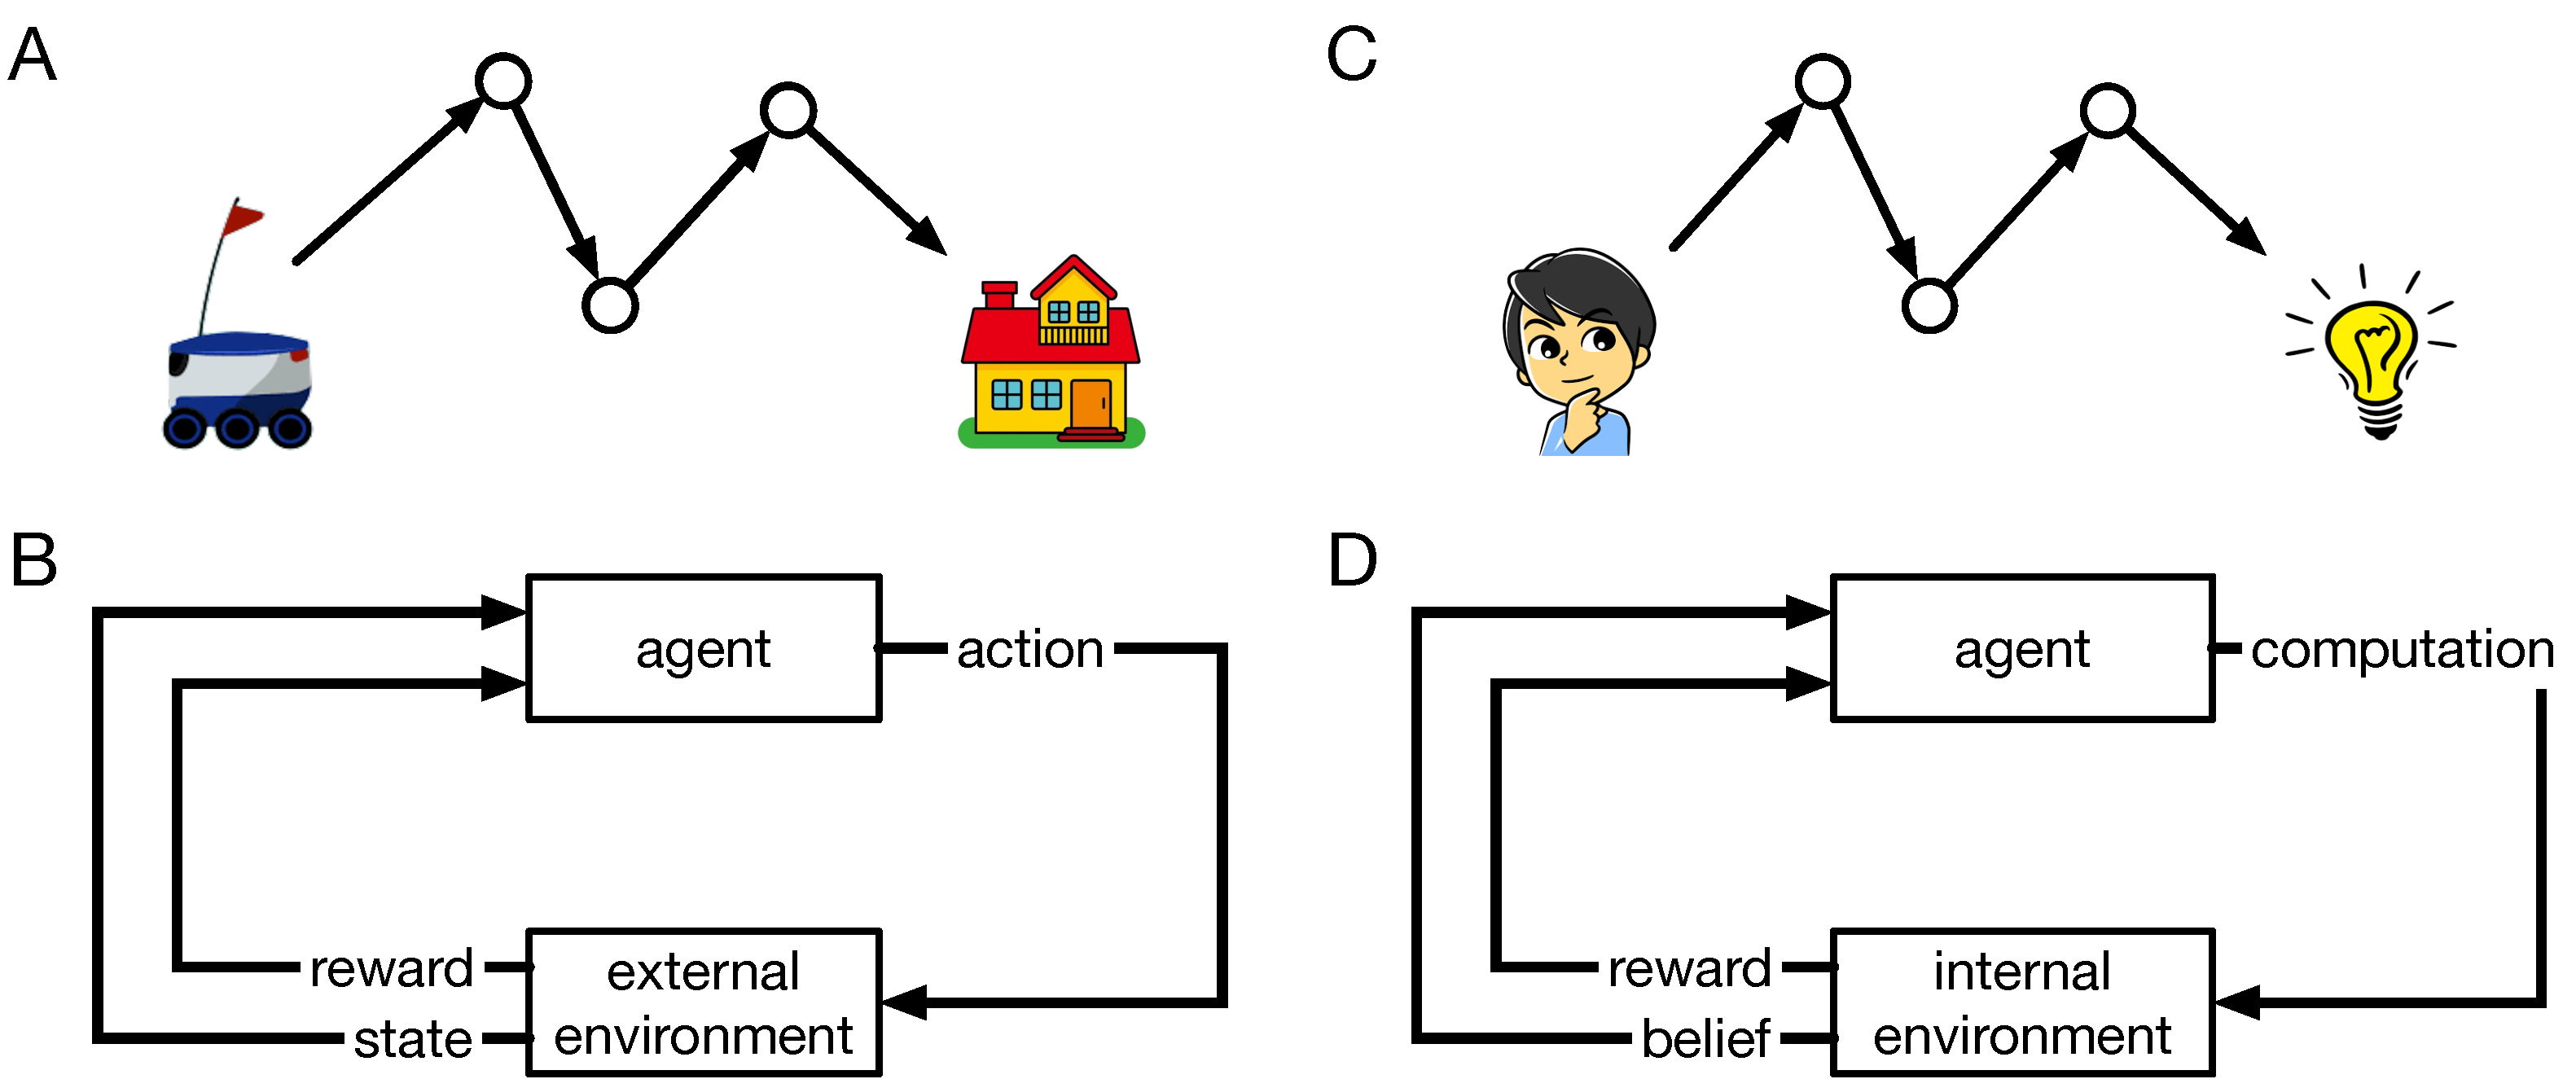
\includegraphics[width=0.9\textwidth]{diagrams/sequential-intuition.pdf}
  \caption{Sequential decision problems posed by external and internal environments.}
  \label{fig:sequential-intuition}
\end{figure}

\figref{fig:sequential-intuition}{c} illustrates a seemingly very different type of situation: a person trying to come up with a solution to a difficult problem. However, as the diagram suggests, the two cases actually share the same basic structure. Both involve an extended interaction between an agent and an environment; but whereas the robot is interacting with an \emph{external} environment, the thinker is interacting with an \emph{internal environment}: their own mind. Just as the robot makes several moves, and visits several locations before reaching the destination, the thinker has several thoughts, and enters several mental states before discovering the solution. Indeed, as illustrated in \figref{fig:sequential-intuition}{d}, this problem can be modeled in precisely the same way as the delivery problem. However, now the actions correspond to computations (thoughts) and the states correspond to beliefs (mental states). Thinking changes one's mental state just as moving changes one's physical state; and it also incurs a cost---at the very least, thinking takes time.

An important property of sequential decision problems is that there is often a dissociation between the short-term reward and the long-term \emph{value} of performing some action. For example, if the robot had the option of simply sitting still, this would incur no cost and would thus be the most rewarding action in a myopic sense. However, the potential for the large reward associated with making a delivery makes paying this cost worthwhile. Thus, moving has value. By the same token, a truly myopic agent (one who only considers immediate rewards) would never do any thinking at all! Thinking only has value insofar as it can inform our future behavior.\footnotemark{}

\footnotetext{Note that, subjectively, thought itself can be rewarding (sometimes intensely so; \citealp{gopnik1998explanation}). However, just as with ``secondary reinforcers'' like money, this is not because thought is inherently valuable, but because it is associated with value. Nevertheless, this association may be deeply engrained, perhaps even genetically so. We return to this question in the conclusion.}

The power of identifying this parallel between external and internal environments is that it allows us to leverage existing knowledge about sequential decision problems (a substantial chunk of AI research) to build rational mechanistic models of cognition. That is, we can apply the same formalisms and algorithms that might help a robot deliver groceries to instead characterize the problem of resource-bounded cognition, and identify cognitive processes that optimally solve that problem.

\section{The shoulders of giants}

Our approach builds on a long history of work in artificial intelligence and cognitive science. Formally, our approach draws heavily on concepts and tools developed in \emph{rational metareasoning}, a subfield of artificial intelligence that aims to construct artificial agents that make effective use of their limited computational resources \citep{russell1991principles,hay2016principles}. Indeed, in many ways, our approach is simply the application of these ideas to understand human cognition. At the same time, many of these ideas have parallels in cognitive models, and still more can be traced to the period before the boundary between cognitive modeling and artificial intelligence was well-defined. Below, we review these ideas from a psychological perspective, noting the parallel concepts in AI when relevant. Ultimately, we will synthesize these key insights into a formal definition of rational mechanistic models of cognition.

% cognition is \emph{dynamic} (sequential, occuring over time), \emph{bounded} (subject to costs or constraints), and \emph{optimized} (maximizing utility). As illustrated in Table~\ref{tab:comparison}, various combinations of these assumptions are made frequently in models of the mind. However, by capturing all three ideas at once, the current approach has advantages that cannot be achieved with any subset.

\subsection{Optimal models of cognition}\label{sec:intro-optimal}

What does it mean, formally, for a cognitive model to be rational? Following \citet{anderson1990adaptive}, we formalize rationality in terms of \emph{optimality}. A model of a cognitive process (henceforth just ``a cognitive process'') is optimal if it performs a cognitive function as well as it possibly could. More precisely, an optimal cognitive process is one that produces the maximum value of an \emph{objective function}, out of a set of possible models:
\begin{equation}\label{eq:intro-optimal}
  π^* = \argmax_{π \in \Pi} U(π).
\end{equation}
Here, $U$ (for utility) is the objective function, and each $π \in \Pi$ is a possible cognitive model. Defining an optimal cognitive model thus amounts to specifying the function or goal of the cognitive process (through $U$), and the set of possible processes (through $\Pi$).

Perhaps the most fundamental optimal model is expected utility theory, which states that one should select actions that yield the best outcomes in expectation (i.e., on average). Given that the world is in state $w$, the action with maximal expected utility is defined as
\begin{equation}\label{eq:eut}
  a^*_w = \E_{o \mid w, a} U(o),
\end{equation}
Although it was not originally conceptualized in this way, we can think of expected utility theory as an optimal model where the set of possible cognitive processes $\Pi$ contains all possible mappings from world states to actions and the utility function is defined as
\begin{equation}\label{eq:perfect}
  U(π) = \E_{o \mid \pi} [U(o)] = 
  \E_{w} \left[
    \E_{a \sim \pi(w)} \left[
      \E_{o \mid w, a} U(o)
    \right]
  \right].
\end{equation}
That is, choosing actions according to expected utility theory yields the highest utility outcomes, on average. In rational metareasoning, maximizing $U$, as defined in Equation~\ref{eq:perfect}, is known as \emph{perfect rationality} \citep{russell1997rationality}.\footnote{%
  More precisely, perfect rationality is usually defined in terms of the total utility attained over the agent's lifetime, and it accounts for limits on the information available to the agent (i.e., not knowing $w$). 
  % Equation~\ref{eq:perfect} describes the special case where the agent makes a single choice and has perfect information.
}

Expected utility theory is the foundation of modern (neoclassical) economics, allowing analysts to predict aggregate market behavior by assuming that each individual maximizes their own welfare. But it is so abstract that it initially seems to tell us little about cognition itself. Nevertheless, applying the optimization principle in more constrained domains (perhaps implicitly) has yielded important insights about many areas of cognition, including perception \citep{marr1982vision,knill1996perception,najemnik2005optimal} categorization \citep{anderson1991adaptive,ashby1995categorization,tenenbaum2001generalization}, memory \citep{anderson1989human}, and language \citep{goldwater2009bayesian}.

The power of optimization as a tool for cognitive modeling is that it makes decisions for us. That is, it reduces the amount of flexibility we have when specifying a model. This may sound like an impediment---and indeed, it sometimes feels that way---but it can have enormous benefits. Conceptually, optimality is a source of intuition. Cognitive processes can be very complex, and simply observing what people do and trying to reason backwards to how they do it can be challenging---especially if we want to understand \emph{why} they do it that way. Exploring optimal solutions, even when they don't explain human behavior especially well, helps us understand the function of cognitive processes, which in turn helps us generate hypotheses about how those processes actually work.

From a statistical perspective, optimality acts as an inductive bias. Any given behavioral phenomenon is consistent with countless cognitive models \citep{anderson1978arguments}, but only a small subset of those are optimal. If people are well-adapted to their environment, then all else being equal, the optimal models are more likely to resemble the truth than an arbitrary alternative model. Of course, people are not perfectly adapted to their environment; thus, one can always achieve a more accurate model of a particular phenomenon by abandoning the assumption of optimality. But when data are limited, or we are exploring a domain we know very little about, or we want to generalize our predictions in non-trivial ways, having a constraint that is \emph{mostly} true can improve our chances of making predictions that are \emph{mostly} accurate.

Problems arise, however, when optimality isn't even mostly true. And there are many settings where that seems to be the case. To take just one example, recall that according to expected utility theory, one should take actions that yield the highest utility outcomes in expectation. This seems straightforward enough, right? Not for humans. People systematically violate expected utility theory, making choices that cannot be reconciled with any utility function \citep{allais1953comportement,ellsberg1961risk,kahneman1979prospect}. Since then, and to this day, a major focus in research on human decision-making has been to characterize exactly how and why people violate expected utility theory, for example because they misperceive the probabilities involved \citep{kahneman1979prospect} or don't consider the different actions independently \citep{roe2001multialternative}.

\subsection{Accounting for constraints}\label{sec:intro-constraints}

Herb Simon \citeyearpar{simon1955behavioral} famously offered a different type of explanation for people's failure to maximize utility: People don't maximize Equation~\ref{eq:perfect} because that's not the problem they're actually faced with. In most real-world problems, there are many actions, and each action could result in many different outcomes. Considering every possible outcome of every possible action each time we are faced with a decision would be paralyzing. Not to mention, the utility of an outcome is itself a complicated thing to evaluate (potentially requiring one to consider the action one would take next given that outcome) and we might not know the exact state of the world (either because the information isn't available or because we simply didn't take note of it). For decisions of the complexity that people face every day, even the largest supercomputers would be completely unable to evaluate expected utilities as in Equation~\ref{eq:eut}. For a person to attempt to do so, using a biological computer that uses less power than an incandescent lightbulb, wouldn't just be hopeless---it would be irrational. 

This notion, that our choices reflect not only the expected utility of their outcomes, but also our limited ability to compute those utilities is called \emph{bounded rationality} \citep{simon1990bounded}. More generally, Simon suggests that human cognition---and the very definition of rational behavior---is shaped by  both ``the structure of task environments and the computational capabilities of the actor'' \citep{simon1990invariants}. By accounting for those constraints as part of the definition of the problem that people have to solve (as opposed to a flaw in the solution), we can continue to apply the rationality principle in cases where computational constraints render perfect rationality (Equation~\ref{eq:perfect}) unattainable.

In modern psychological research, Simon's ideas are reflected in many different ways. One of the most prevalent is the notion of \emph{ecological rationality} \citep{gigerenzer1999simple,goldstein2002models,todd2012ecological}. Ecological rationality is based on the idea that people make decisions using simple, but adaptive heuristics. These heuristics are computationally ``frugal'', meaning that people can actually apply them in the real world. But critically, they result in good decisions most of the time. How is this possible? The answer lies in the \emph{ecological} of ecological rationality. The heuristics people use would not produce good results in any hypothetical world---they produce good results in \emph{our} world. To understand this formally, ecological rationality emphasizes the distribution over the world state $w$ in Equation~\ref{eq:perfect}. The overall utility of a cognitive process is mostly determined by the behavior it produces in high-probability states.


Proponents of ecological rationality take a strong stance against the notion of optimality, suggesting that optimization taking into account cognitive contraints is ``demonic'' (\citealp{gigerenzer1999simple}; Chapter~1).

% While the importance of bounded rationality and ecological adaptation is widely accepted, the implications of Simon's ideas for optimal modeling are more controversial. Proponents of ecological rationality take a hard stance, calling optimization ``demonic'' (\citealp{gigerenzer1999simple}, Chapter 1). Indeed, clearly people's cognitive processes are not optimal in the sense of maximizing utility (Equation~\ref{eq:eut2}), and nor are they likey to be exactly optimal in the cons

%sub \section{Resource-rationality}\label{sec:intro-XX}


Clearly bounded rationality is a more appropriate benchmark in many cases, but it lacks some of the precision of optimality. To regain that precision while capturing Simon's key insight, we can explicitly formalize the role of cognitive constraints within the optimality paradigm. One very natural way to do this, proposed by \citet{lewis2014computational} and \citet{griffiths2015rational}, is to formalize bounded rationality as \emph{bounded optimality}. Horvitz \citeyearpar{horvitz1987reasoning} defines bounded optimality as ``the optimization of computational utility given a set of assumptions about expected problems and constraints on resources'' (compare to Simon's ``structure of task environments'' and  ``computational capabilities''). \citet{russell1995provably} provide a more formal definition of bounded optimality as a property of a program, namely that it yields the maximum expected utility when executed on the agent's computational architecture, or ``brain'' $B$. We can thus define a bounded optimal cognitive process as
\begin{equation}\label{eq:bo}
  π^\text{BO} = \argmax_{π \in \Pi_B} \E_{o \mid \pi, B} [U(o)],
\end{equation}
where $\Pi_B$ is the set of all cognitive processes that can be executed by brain $B$ and $\E_{o \mid \pi, B} [U(o)]$ is the expected utility of the outcome that results from executing process $\pi$ on brain $B$.

As a definition of rationality for cognitive processes, bounded optimality is intellectually ideal, but problematic in practice. It is ideal because it exactly defines the problem that a resource-contrained agent faces.
% the objective that an optimal cognitive process should optimize. 
In pratice, however, it is very difficult to identify bounded optimal cognitive processes. There are two reasons for this. First, it requires optimizing over the set of all cognitive processes a brain could execute. It is not clear how one would specify this set, let alone find the optimum. Second, bounded optimality is not really a property of cognitive processes and outcomes; it is a property of entire minds and lifetimes.\footnote{%
  Below, we focus on the process/mind problem. The outcome/lifetime problem---that is, that the utility of an outcome depends on the future outcomes that it permits or precludes---can can be addressed by the notion of long-term value (briefly described in Section~\ref{sec:intro-intuition} and formalized in Chapter~\ref{sec:formalism}). That is, we can define the utility of an outcome in terms of both the immediate and future rewards it yields.
} Different cognitive processes all draw on the shared resources of one brain. Thus, we cannot identify the optimal process for one particular cognitive function without considering the effect it has on all the other functions the brain must support. That is, bounded optimality seems to prevent us from decomposing the monolithic problem of characterizing ``rational cognition'' into a set of more manageable problems of characterizing specific rational cognitive processes.

Fortunately, these two challenges are not entirely insurmountable. We address the problem of specifying possible processes in Section~\ref{sec:intro-sequential}, and optimization in Chapter~\ref{sec:formalism}. The challenge of decomposability is addressed in the next section.

\subsection{The cost and value of mental actions}\label{sec:intro-utility}

One of the key challenges of applying bounded optimality is that the optimization occurs over the agent's entire brain. We use our brains for many different things, and have to decide how much mental resource to allocate to each. When viewed as a single constrained optimization problem, this is intractable, as it requires jointly solving for the optimal cognitive process for all the different problems our brain has to solve.

As defined in Equation~\ref{eq:bo}, bounded optimality poses a single constrained optimization problem, where we must identify a single cognitive process that solves all the problems the agent might face, using a single shared resource, the brain. This is an intimidating problem, to say the least. Perhaps, however, this is not the only way to view the problem. Consider another case where an animal must allocate a finite shared resource amongst several different activities: foraging. Rather than allocating mental resources across different cognitive functions, the animal must allocate their time across different patches where food might be found. Initially, this problem seems very challenging because the correct amount of time to allocate to each patch depends on the time allocated to every other patch. But as shown by \citet{charnov1976optimal}, the optimal solution is actually quite simple: stay in a patch as long as the rate of food intake is more than what you could expect to find elsewhere (the average rate of intake, learned over experience). More generally, one should allocate resources to an activity as long as the utility gained from that activity exceeds the \emph{opportunity cost} of not allocating those resources to some other activity. As brilliantly observed by \citet{kurzban2013opportunity}, this principle applies equally to the allocation of cognitive resources.

Leveraging the insight that thinking carries an opportunity cost, \citet{lieder2018bounded} showed that we can characterize the utility of specific cognitive processes as an additive combination of outcome utility and cognitive cost,
\begin{equation}\label{eq:resource}
  U(\pi) = \E_{o \mid \pi} [U(o)] - \cost(\pi),
\end{equation}
where cost captures the opportunity cost of the resources consumed by $\pi$. 
\citet{lieder2018bounded} present a derivation of this cost in terms of the time that different resources are allocated, but more nuanced factors related to the neural implmentation of cognitive processes in humans are likely at play as well \citep{musslick2021rationalizing}.

Of course, the notion that cognition is costly or effortful goes back much further than this link to bounded optimality. Indeed, simple introspection suggests that that thinking is effortful, and therefore costly in the same way as carrying heavy groceries is.\footnote{%
  Of course, it is not hard to see how the perceived cost of carrying groceries is itself ultimately a form of opportunity cost, i.e., the other bodily procesess those calories could have been burned to support.
} Thus, a long history of work has studied how people balance outcome utility and cognitive cost (see \citealp{shenhav2017rational} for a review). One critical insight from this work is that the optimal point on this trade-off is not always the same. For important decisions with clear factors to consider, thinking a lot is often worthwhile. For unimportant decisions, or ones that are too complex to effectively reason about, the benefit of thinking a lot is unlikely to outweigh the cost.

The idea that one should allocate different amounts of mental effort in different situations has been formalized in many different ways \citep{shenhav2013expected,anderson1990adaptive,lieder2017strategy}. However, all these different approaches draw on a key insight. The choice of how much effort to allocate (or more generally, which cognitive process to use) is analogous to the choice of which action to take in the world. Accordingly, just as expected utility theory defines the optimal action to take in any world state (Equation~\ref{eq:eut}), we can define the optimal cognitive process to use in any given world state as
\begin{equation}\label{eq:process-world}
  π^*_w = \E_{o \mid w, π} U(o) - \cost(w, π).
\end{equation}


% as we can define the utility of an \emph{action} as the expected utility of the outcome it produces, we can define the utility of a \emph{cognitive process} as the expected utility of the outcome \emph{it} produces cognitive cost. This yields:
% \begin{equation}\label{eq:evc1}
%   U(w, c) = 
%     \E_{o \mid w, c} \left[
%       U(o)
%     \right] - \cost(c)
% \end{equation}
% where $c$ corresponds to a ``cognitive action''. 

% Defining the utility of cognitive actions in this way allows us to define a bounded optimal cognitive process as a mapping from states to cognitive actions that always maximizes $U(w,c)$, just as a perfectly optimal process maximizes $U(w,a)$.
% \begin{equation}
%   \pi^*(w) = \argmax_c U(w, c)
% \end{equation}


% We will refer to decision, those concerning the allocation of mental resources, as \emph{metalevel decisions}. This is contrasted with 



The content and interpretation of $c$ in Equation~\ref{eq:evc1} varies substantially across different instantiations of this general principle. One influential example is the \emph{expected value of control} (EVC) \citep{shenhav2013expected}. In EVC, $c$ corresponds to a \emph{control signal}, which modulates the behavior of a simpler cognitive process. In the simplest case, the control signal is a scalar indicating how much effort is invested into performing a task. In more complex cases, the control signal can have multiple dimensions, controlling not the quantity but also the nature of cognitive effort exerted \citep{musslick2015computational,grahek2020computational,ritz2021cognitive}.

In another instantiation of this principle, $c$ corresponds to a \emph{strategy} for solving a problem. A classic example is the decision of whether to use a ``model-free'' or ``model-based'' strategy; intuitively, a model-free strategy relies on habits or learned associations, while a model-based strategy involves explicit reasoning about the consequences of one's actions. In an early application of this idea, \citep{daw2005uncertaintybased} recognized that each system will yield better actions under different circumstances (emphasizing the $U$ term in Equation~\ref{eq:evc1}) suggesting that people choose their strategy accordingly. Expanding on this, later work showed that people are also sensitive to the different costs of the two systems \citep{keramati2011speed,kool2017costbenefit} and that they can use strategies that combine model-based and model-free reasoning \citep{keramati2016adaptive,huys2015interplay}. Much of this work only makes an intuitive appeal to a utility-cost tradeoff. More recently, \citet{lieder2017strategy} presented a model of strategy selection that explicitly optimizes an expression analogous to Equation~\ref{eq:evc1}, showing that it can explain when people use different strategies for deciding between options that vary along many dimensions.

This last example highlights an important feature of all the models discussed in this section: Although the \emph{selection} of a control signal or strategy is a single event, the ultimate outcome is determined by ... a sequence.

% For our purposes, however, there is one important difference between EVC and VOC, or more generally, between cognitive control and strategy selection. In the latter case, the cost of executing a strategy is typically assumed to be directly related to the \emph{amount} of computation that is performed. More precisely, the cost of applying a strategy depends on the number of discrete computational operations it performs, and the time that each operation takes \citep{payne1988adaptive}. It is possible to decompose the cost of a strategy in this way because strategies are \emph{sequential}.


% \footnote{%
%   Note that we depart from the original definition of EVC \citep{shenhav2013expected} for consistency with the other equations in this section. In the original definition, the utility is defined in terms of the outcome of the process, rather than the behavior iteself. Non-trivially, the outcome was proposed to include the following world state, making EVC a sequential framework. However, most applications of EVC do not actually use this feature, assuming that the utility of the outcome depends only on the behavior in the current trial, as in Equation~\ref{eq:evc1}. One notable exception is the visual attention model in \citet{lieder2018rational}, which employs an early version of the framework proposed here.
% } 

% What is the optimal cognitive process according to EVC? Interestingly, there are two ways to answer this question. On one hand, we can think of the control signal itself as the cognitive process. Indeed, in applications of EVC, the control signal often parameterizes an evidence-accumulation process (the DDM, described in the next section; \citealp{musslick2015computational,grahek2020computational}). Thus, selecting a control signal amounts to selecting a cognitive process to execute. Formally, this corresponds to defining $π = c$ and $U(w, π) = \text{EVC}(w, π)$.This results in our general definition of optimal cognitive processes in Equation~\ref{eq:intro-resource}, with the addition that the utility of the process (i.e., the value of the control signal) depends on the state of the world (e.g., whether the current trial is easy or hard).

% Alternatively, we can think of the optimal cognitive process as the strategy for selecting control signals, that is, by maximizing EVC. In this case, we would define the utility of the selection strategy as
% \begin{equation}\label{eq:evc2}
%   U(π) = \E_w \left[
%     \E_{c \sim π(w)} \left[
%       \E_{a \mid c, w} \left[
%         U(w, a)
%       \right] - \cost(c)
%     \right]
%   \right],
% \end{equation}
% where $π$ is now the mapping from world states to control signals. Clearly the mapping which maximizes Equation~\ref{eq:evc1} in all states will also optimize Equation~\ref{eq:evc2}. Thus, as long as we do not put any constraints on the space of selection strategies, the definitions are equivalent. Conceptually, however, the notion of a cognitive process whose function is to select cognitive processes (a \emph{metalevel} process, perhaps) is critical.


% Importantly, however, this reduction can only be applied under the assumption that all conceivable representational mappings are actually possible. By making stronger, psychologically motivated, assumptions about the form of the cognitive process (the mapping), we can still glean interesting cognitive insights. For example, \citet{bhui2018decision} use 

% \begin{equation}\label{eq:intro-resource}
%   π^* = \argmax_{π \in \Pi} U(π) - \cost(π),
% \end{equation}

% Conceptually $U$ and cost are distinct, referring to external and internal concerns, respectively. However, because both are ultimately a function of the cognitive process, we could just as well include cost within the $U$ function. Thus, at the end of the day, resource-rational models are really optimal models with a specific kind of objective function (and perhaps also a more limited set of possible models $\Pi$).

\subsection{Information and representation}\label{sec:intro-info}

One of the most common choices for the cost function is based on information theory. In these models, the cognitive process forms a \emph{representation} of the state of the world, which then informs the action that is taken. The heart of the cognitive process here is the (probabilistic) mapping from world states $w$ to mental representations $m$. The utility of this mapping is defined as
\begin{equation}\label{eq:intro-info}
    U(π) = \E_w \left[
      \E_{m \sim π(w)}[U(w, a_m)]
    \right] - I_π(w, m)
\end{equation}
where $a_m$ denotes the action taken given representation $m$, $U(w, a_m)$ is the utility of taking that action in the world state $w$, and $I_π(w,m)$ denotes the \emph{mututal information} between the state of the world and the representation under the mapping $π$. Intuitively, $I$ captures the fidelity of the representation. There are two key ideas to take away from this equation. First, cognitive processes can produce intermediate mental states, which are used to select actions. Second, both the action utility and cost depend on the mental state, and these two forces are in a fundamental conflict. A precise representation of the world allows one to select good actions, but such representations are costly to form.

Information-theoretic models of this sort are commonly used in the study of perception \citep{sims2016rate} and memory \citep{gershman2021rational}, most frequently their intersection. In this literature, the models are typically cast in the language of \emph{rate-distortion theory}. Here, the utility function captures the discrepancy between the stimulus $w$ and a reconstruction of that stimulus $a_m$ based on the remembered perceptual representation $m$. In a classic application of this approach, \citet{sims2012ideal} showed that a model that flexibly allocates informational resource across an arbitrary number of items explains human reconstructions better than a classic model with a fixed number of working memory slots. More recent work showed that people can strategically prioritize more important dimensions of the stimulus (that is, they are sensitive to $U$; \citealp{yoo2018strategic}) and can also allocate more or less resource in total \citep{berg2018resourcerational}. This latter result is interesting because it supports an additive cost like in Equation~\ref{eq:intro-info} over a fixed but costless capacity constraint.\footnote{
  Typically, rate-distortion models are expressed in terms of such a fixed constraint, i.e., maximizing utility subject to a constraint on mutual information. However, because mutual information is an expectation over values of $x$ and $w$, one can find a multiplier on the cost that results in any given average level of expectation (the Lagrange multiplier; see \citealp{ortega2013thermodynamics}).
} Beyond memory, rate-distortion models have also been used to explain the exponential shape of people's generalization curves (\citealp{sims2018efficient}; c.f. \citealp{shepard1987universal} and scalar variability in approximate number representation (\citealp{piantadosi2016rational}, c.f. \citealp{fechner1860elemente}).

In economics, information-theoretic models go under the name \emph{rational inattention}, reflecting the idea that one's mental representation is the result of ignoring features of the world that aren't important to one's decision \citep{sims1998stickiness,caplin2013behavioral}. 
% This idea was initially developed by \citet{sims1998stickiness} to understand why prices don't respond to changing market conditions as quickly as expected-utility-based models predict. List a few findings... 
One interesting result from this literature is that, for the commonly used mutual-information cost function, the optimal cognitive process has exactly one representation for each possible action; that is, there is a one-to-one correspondence between $a$ and $m$. This allows one to eliminate $m$ entirely, yielding a reduced form model in which the cost is simply the mutual information between state and action \citep{matejka2015rational}, as proposed in free-energy based models \citep{friston2010freeenergy,ortega2013thermodynamics}. However, while this reduction is mathematically fascinating, if our goal is to define rational \emph{mechanistic} models of cognition, we seem to be going backwards. By eliminating the mental representation from the model, we end up with a more sophisticated form of behaviorism, where we attempt to understand a cognitive process simply as a mapping from stimulus to response.

%  Ultimately, the result is a slight variation of the commonly used ``softmax'' model of choice,
% \begin{equation}
%   \pi(a \mid w) \propto \expp{\frac{1}{λ} \cdot (U(w, a) + \alpha_a)}
% \end{equation}
% where $\lambda$ is a scaling constant on the mutual-information cost and $\alpha_a$ captures a default tendency to take action $a$ (the values of $\alpha$ can be determined optimally, being larger for actions that have higher average utility).
% This reduction is mathematically fascinating, and it provides a useful extension of the standard softmax model by accounting for the habitual tendency to take actions that are usually good. 
% However, if our goal is to define rational \emph{mechanistic} models of cognition, we seem to be going backwards. By eliminating the mental representation from the model, we end up with a more sophisticated form of behaviorism, where we attempt to understand a cognitive process simply as a mapping from stimulus to response.

Thus, information-theoretic models are well-suited for explaining how we represent the world and why we behave somewhat randomly. But they are perhaps less ideal for understanding the mechanisms that generate those representations or yield that randomness. Nor is it clear how to apply these models in cases where the cost is not naturally cast in terms restricted information flow.

\subsection{The sequential nature of thought}\label{sec:intro-sequential}

The fact that cognitive processes are sequential, in the sense that they occur over time rather than all at once, is self-evident. Thus, some notion of sequentiality is an essential feature of a model that captures cognitive mechanisms at any level of detail. Here, however, we will use a slightly more restrictive notion of sequentiality. Specifically, we take sequentiality to mean that cognitive processes can be broken down into a sequences of \emph{elementary information processes} \citep{simon1979information,posner1982information,chase1978elementary}, or simply, cognitive operations.

One widely used class of sequential models are \emph{evidence accumulation} models (also called ``sequential sampling models''), such as the drift diffusion model (DDM; \citealp{ratcliff1978theory}), leaky competing accumulators \citep{usher2001time}, and decision by sampling \citep{stewart2006decision}. According to these models, decision making involves accumulating noisy evidence in favor of each possible choice until the evidence for one choice is sufficiently greater than the evidence for the other(s). That is, the cognitive process can be understood as a sequence of operations, each of which accumulates a small amount of evidence. In their simplest form, there is only one type of operation; these models can explain not only the choices we make (including when we make mistakes), but also how long it takes to make those choices. More complex evidence accumulation models take into account the possibility of attending to different sources of information, such as different options \citep{krajbich2010visual} or attributes \citep{russo1983strategies}; these models can account for (if not predict) additional data such as what we look at when making a decisision, and they can account for systematic deviations from expected utility \citep{busemeyer2019cognitive}.
% For example, these models predict that easier decisions will be made both more consitently and more quickly, and that mistakes will be faster than correct choices.

Another important class of dynamic models, \emph{cognitive architectures}, aims to capture a more diverse range of mental activities, beyond simply accumulating more evidence. Cognitive architectures, most notably ACT-R \citep{anderson1996act} and SOAR \citep{laird1987soar}, explicitly model individual cognitive operations such as perceptually encoding a stimulus, recalling information from memory, and transforming symbolic reprenstations the world. These models can trace their intellectual roots to the infancy of artificial intelligence research \citep{newell1956logic}, where the discovery that digital computers could solve complex problems by breaking them down into a sequence of very simple operations led to the hypothesis that a similar principle might underlie human intelligence \citep{newell1958elements,newell1972human}. 
% The core assumption of these models is that all cognitive processes can be broken down into so-called \emph{elementary information processes} \citep{simon1979information,posner1982information,chase1978elementary}.

Formally, we can define sequentiality as a restriction on the space of possible cognitive processes, $\Pi$. Intuitively, the cognitive process corresponds to a strategy for selecting cognive operations. But how should this be strategy be specified? Initially, we might be tempted to say that a cognitive process is simply a sequence of cognitive operations. But this assumes that a given cognitive process will always execute the same sequence of operations, regardless of the state of the world. Perhaps the cognitive process should be a mapping from world states to (distributions over) sequences of operations?. This is a valid approach, but it retricts the cognitive process to be ``open loop'' in the sense that it cannot reactively adjust which operations it performs based on the effects of previous operations, which are typically stochastic. To capture a more adaptive form of ``closed loop'' strategy, we can instead define a cognitive process in terms of a mapping from \emph{mental} states to single cognitive operations (for simplicity, we assume a deterministic mapping). Thus, each $π \in \Pi$ is defined as a function, $\pi: \M \rightarrow \C$, such that
\begin{equation}\label{eq:intro-sequential}
   c_t = \pi(m_t)
\end{equation}
That is, at each time step, $\pi$ chooses the next cognitive operation to execute given the current mental state. For example, consider the DDM, which assumes that evidence is accumulated until the total evidence hits an upper or lower threshold, $b$ or $-b$. We could formalize this strategy as the function
\begin{equation}
  \pi(m) = \begin{cases}
    \text{choose A} &\text{if } m > b  \\
    \text{choose B} &\text{if } m < -b  \\
    \text{draw sample} &\text{if } -b ≤ m ≤ b
  \end{cases}
\end{equation}

Formalizing a cognitive process in this way provides a natural way to define the cost of executing a strategy, as the sum of the cost of each operation it executes:
\begin{equation}\label{eq:intro-cost}
  \cost(π) = \E_w \left[
    \E_{\cseq \mid \pi} \left[
      \sum_t^N \cost(c_t)
    \right]
  \right].
\end{equation}
where $\cseq = (c_1, c_2, \ldots, c_N)$ is a sequence of cognition operations.
This may look like kicking the can down the road, but defining the cost of a strategy as the sum cost of all the operations it executes represents real progress. This is because operations are much simpler objects than strategies, and so their cost can be more easily estimated \citep{donders1969speed}. Even without empirical measurement, very simple assumptions (e.g. that all operations have the same cost) can yield useful predictions. For example, using this assumption, \citet{payne1988adaptive} analyzed the cost and expected action utility of a set of ten possible decision strategies, finding that people used strategies that struck good cost-benefit tradeoffs, adapting their choice of strategy to time constraints and the structure of the decision problems.

On the other hand, formalizing cognitive processes as mappings from mental states to cognitive operations poses considerable challenges. Many models have a very large space of possible mental states, and we need to specify which cognitive operation is executed in each one. If there are $M$ possible mental states and $C$ possible operations, there are $C^M$ possible mappings. If $M$ is large (and it often is), this results in a huge space of possible cognitive processes. Searching this entire space is effectively impossible. Payne et al. circumvented this problem by manually specifying a small set of candidate strategies (mappings). But how can we be sure that this set includes the strategies people use, or that achieve the best cost-benefit trade-offs? Indeed, as shown by \citet{howes2009rational}, failing to consider all the possible strategies can yield incorrect conclusions about which cognitive architectures are consistent with a given pattern of behavioral data. But as the set of strategies grows, more and more architectures become consistent with the data. As Howes et al. convincingly argued, adopting additional constraints---specifically, the assumption of optimality---may be necessary to distinguish between candidate architectures.

% Constructing dynamic models poses a substantial challenge, however, particularly when there are many different elementary operations. Because any number of cognitive operations can be executed at any time, one must not only specify the set of operations and their effects, but also a strategy for how the operations are chosen \citep{payne1988adaptive}. In practice this is often done in an ad hoc manner (c.f., \citealp{howes2009rational}).

% \begin{equation}
%   \cost(π) = \expect{\sum_t \cost(c_t)}{c_t \sim π}
% \end{equation}

\pagebreak

\subsection{Optimal sequential models}\label{sec:intro-final}

\definecolor{optimal}{HTML}{e41a1c}
\colorlet{simon}{SchoolColor}
\definecolor{utility}{HTML}{4daf4a}
\definecolor{info}{HTML}{377eb8}
\definecolor{sequential}{HTML}{7B2FB0}
% \definecolor{cost}{HTML}{D4609A}


\newcommand{\hl}[2]{%
  {\color{#1!90!black} #2}
}

\newcommand{\specialitem}[2]{%
  \item[%
    {\color{#1} \textbf{#2}}%
  ]
}

Having defined and briefly reviewed optimal and dynamic models, we now turn to the key question: How can we define a model that is optimal, resource-constrained, and sequential? To do so, we combine five key insights from the literature reviewed above.
%
\begin{enumerate}
  \specialitem{optimal}{1} An optimal cognitive process is one that maximizes an objective function (Section~\ref{sec:intro-optimal}).
  %
  \specialitem{simon}{2} Cognitive processes are shaped by the structure of both the external environment and the internal environment (Section~\ref{sec:intro-simon}).
  %
  \specialitem{utility}{3} The utility of a mental action depends on its effect on behavior as well as its cost (Section~\ref{sec:intro-utility}).
  %
  \specialitem{info}{4} The behavior produced by a cognitive process is mediated by the mental state it produces (Section~\ref{sec:intro-info}).
  %
  \specialitem{sequential}{5} A cognitive process can be broken down into a sequence of mental operations, with each operation selected based on the current mental state (Section~\ref{sec:intro-sequential}).
\end{enumerate}%
Combining these ideas, yields the following definition of an optimal sequential cognitive process:
%
\begin{equation}\label{eq:intro-master}
  π^* = \hl{optimal}{\argmax_{π}}\ 
    \E \left[
      \hl{utility}{U}(\hl{simon}{w}, \hl{info}{\text{act}(m_t)})
      \ - \sum_t \hl{utility}{\cost(c_t)}
      % \ - \hl{sequential}{\sum_t} \hl{utility}{\cost(c_t)}
      \ \middle\vert\ \hl{sequential}{c_t \sim \pi(m_t)},
      \ \hl{simon}{m_{t+1} \sim T(m_t, c_t, w)}
    \right]
\end{equation}
That is, the optimal cognitive process is a way of selecting cognitive operations that, when applied to the types of problems people encounter, yields a mental state from which high utility actions can be taken, while at the same time minimizing the total cost of those operations. The equation is certainly complex; but as the tacky coloring reveals, none of these ideas are new.

The idea to combine these ideas is not especially new either. In particular, there is a long history of modeling optimal speed-accuracy tradeoffs using evidence accumulation models like the ones described in the previous section. Much of this work can be traced back to the \emph{sequential probability ratio test} (SPRT), which specifies the optimal amount of evidence to collect when evaluating simple binary hypotheses \citet{wald1945sequential}. The rule is simple: continue collecting evidence until there a threshold level of evidence is reached either for or against the hypothesis. When samples are very costly, the optimal threshold is often quite low, capturing the response randomness that is hard to explain in unbounded Bayesian models \citep{vul2014one}. On the other side of the spectrum, as both the cost and informativity of each sample fall, the SPRT converges towards the DDM \citep{gold2002banburismus}; the DDM thus inherits the SPRT's optimality properties. In particular \citet{bogacz2006physics} show that, for any given level of evidence coherence (problem difficulty), there is some fixed threshold that maximizes the rate of reward. Under certain assumptions, this is equivalent to maximizing a linear combination of choice utility and cost.\footnote{
  Maximizing reward rate and an additive difference of utility and cost are equivalent in the sense that, for a given decision problem, there is some time cost such that maximizing the reward rate will also maximize the reward minus cost \citep{wald1948optimum,drugowitsch2012cost}. However, this mapping will vary for problems of different difficulty or stakes. For example, multiplying the payoff for correct decisions by two does not change the optimal reward-rate strategy, but it does change the optimal utility-minus-cost strategy.
} Thus, we can view the DDM as an optimal cognitive process, in exactly the sense defined in Equation~\ref{eq:intro-master}.

The optimality of the SPRT (and by extension, the DDM) depends on the assumption that difficulty and importance of the decision are both known in advance. But this is often not true. By explicitly modeling evidence accumulation as a sequential decision problem, \citet{drugowitsch2012cost} showed that the optimal strategy can still be represented as an evidence threshold when difficulty varies from problem to problem, but this threshold changes over time (rapidly expanding and then slowly collapsing). Building on this work, \citet{tajima2016optimal} characterized the optimal decision thresholds for value-based choices, where both importance and difficulty depend on the difference in value between the choice options \citep{tajima2016optimal}, and three-alternative choices, where the mental states and thresholds reside in an three-dimensional space (including time). Despite this richness, all the models reviewed so far have assumed a very simple cognitive architecture, in which there are only two possible cognitive operations: gather more evidence, or stop. We consider a more complex case, in which an agent must select among different possible sources of evidence, in Chapter~\ref{sec:attention} (c.f., \citealp{hebert2019rational,jang2021optimal}).

Outside of evidence-accumulation models of decision making, optimal sequential models of cognitive procesess are not as commonly seen. 

hoppe2019multistep
acharya2017human
butko2008pomdp
sprague2003eye

models ...
Howes
POMDP visual search

Sampling as a resource-rational constraint response to Falk's BBS

% \citet{hamrick2015think} 
% \citet{lieder2018anchoring} 




% \begin{equation}
%   π^* = \argmax_{π} \E_w \left[
%     \E_{\cseq \sim π(w)} \left[
%       \E_{m \mid \cseq} \left[
%         U(w, a_m)
%       \right]
%       - \sum_i \cost(c_i)
%     \right]
%   \right].
% \end{equation}


% \begin{equation}
%     π^* = \argmax_{\cseq}\,  U(\cseq) - \cost(\cseq).
% \end{equation}


% \begin{equation}
%   π^* = \argmax_{π} \E_{\cseq \mid π} \left[
%     U(a_n) - \sum_i \cost(c_i)
%   \right]
% \end{equation}
% \begin{equation}
%   π^* = \argmax_{π} \E_{\cseq \mid π} \left[
%     \E_{a \mid \cseq} [ U(a) ] - \sum_i \cost(c_i)
%   \right]
% \end{equation}

% This substitution yields little insight on its own. Specifically, what is the utility of a sequence of cognitive operations? Intuitively, the utility of cognition comes from how it affects our actions. Thus, let $\mathrm{act}_N$ be the action we would take after executing the cognitive process $(c_1, c_2, \ldots c_N)$. Further, we can assume that the cost of each operation is independent. This yields
% \begin{equation}
%     π^* = \argmax_{(c_1, c_2, \ldots c_N)} U(\mathrm{act}_N) - \sum_i^N \cost(c_i).
% \end{equation}
% That is, an optimal sequential cognitive process is one which maximizes the utility of the action that the cognitive process produces minus the total cost of all the operations it performs. We express this intuition more precisely in the following chapter (Equation~\ref{eq:optimal-meta-policy-expanded}).

% problem: this isn't actually sequentially optimal


%sub \section{Alternative approaches for rational mechanistic modeling}

% Having defined and briefly reviewed optimal and dynamic models, we now turn to the main question explored by this disseration. How can we construct rational mechanistic models? The answer proposed here is the construction of optimal sequential models. But before

% This is by no means a new question, nor is this dissertation the first to propose a general framework for constructing such models. In the following sections, we briefly review this past work, with an emphasis on ...

%sub \section{Ecological rationality}\label{sec:intro-XX}





%sub \section{Optimal but not dynamic}\label{sec:intro-XX}




% In this way, resource-rationality is more similar \emph{ecological rationality}, a framework based on the idea that people use computationally frugal heuristics, which are highly effective for the kinds of problem that people actually encounter \citep{gigerenzer1999simple,goldstein2002models,todd2012ecological}. For example, if the other players in an environment are using a wide variety of decision strategies, then a heuristic that ignores the other players payoffs entirely may perform best \citep{spiliopoulos2020map}. However, while proponents of ecological rationality explicitly reject the notion of optimization under constraints (e.g. \citealp{gigerenzer1999simple}, Ch. 1), optimization is at the heart of resource-rational models.



% More recently, the notion of optimality has been extended to account not only for the demands imposed by the external environment but also the demands imposed by our own cognitive limitations \citep{howes2009rational,lewis2014computational,gershman2015computational,griffiths2015rational,lieder2020resourcerational}. This approach dates back to Simon \citep{simon1955behavioral} and has been especially useful in the domain of decision-making, where it has been used to explain both how long people deliberate \citep{bogacz2006physics,drugowitsch2012cost,tajima2016optimal,tajima2019optimal,fudenberg2018speed} and also what people think about \citep{callaway2021fixation,jang2021optimal} while making ``simple'' (i.e., non-sequential) choices. However, to the best of our knowledge, there has been no such analysis in the domain of planning, despite the especially critical role that computational limitations play in this case (but c.f. \citep{sezener2019optimizing,mattar2018prioritized} for closely related efforts, which we discuss further below).



% The use of optimization in cognitive models is more controversial. 


% The basic premise of the approach is that the mind should be well adapted to its environment, through some combination of learning and evolution \citep{anderson1990adaptive}. Optimization simply takes this idea to the logical extreme, assuming that the mind is adapted \emph{as well as possible} to the environment.



% % Dynamic: DDMs.

% % Control: attention, metacognition.

% % Adaptive: rational analysis, economics

% % More interesting are models that capture two of the three properties.

% % Dynamic + Control: cognitive architectures.

% % Dynamic + Adaptive: ???

% % Control + Adaptive: EVC


% % \newcommand{\yes}{\checkmark &}
% % \begin{table}[tb]
% %   \caption{Classification of cognitive models.}
% %   \label{tab:comparison}
% %   \centering
% %   \begin{tabular}{cccc|c}\toprule
% %   Dynamic & Controlled & Optimized & Notable Examples \\
% %   \midrule
% %   \yes & &
% %     DDM 
% %   \\ & \yes &
% %     Attention, metacognition 
% %   \\ & & \yes
% %     Rational analysis, economics 
% %   \\ \yes \yes &
% %     Cogntive architectures, ecological rationality
% %   \\ \yes & \yes 
% %     Bogacz ?
% %   \\ & \yes \yes 
% %     EVC, information-theoretic
% %   \\ \yes \yes \yes
% %     This dissertation 
% %   \\ \bottomrule
% %   \end{tabular}
% % \end{table}


% sampling
% information theoretic
% rational analysis
% ecological rationality
% EVC
% cognitive architectures

% % \begin{table}[tb]
% %   \caption{caption here}
% %   \label{tab:tablename}
% %   \centering
% %   \begin{tabular}{ccc|c}\toprule
% %   Dynamic & Control & Adaptive & Examples \\
% %   \midrule
% %   \yes & &     DDM \\
% %   & \yes &     Attention, metacognition \\
% %   & & \yes     Rational analysis, economics \\
% %   \yes \yes &  Cogntive architectures \\
% %   \yes & \yes  ? \\
% %   & \yes \yes  EVC \\
% %   \yes \yes \yes  This dissertation \\
% %   \bottomrule
% %   \end{tabular}
% % \end{table}



% In comparison to non-rational dynamic models, the proposed approach
% - naturally captures metacognition and control
%   - c.f. aDDM which assumes random attention
%   - c.f. metamemory which ignores control
% - avoids combinatorial search

% Compared with non-sequential rational models, 



%  % the problem posed by the internal environment (what I will call the \emph{meta-level} problem) is exactly analagous to the problem posed by the external environment (the \emph{object-level} problem). 








% In comparison to non-dynamic rational models
% - captures the process/mechanism (c.f. information-theoretic accounts)
% - more optimal
% - captures sequential dependence



% % Taken from planning (cut there?)
% These challenges---hypothesis generation, generalizable prediction, and functional explanation---are not unique to planning; indeed, they arise in nearly all areas of cognition. In many domains, progress in addressing these challenges has been made by analyzing optimal solutions to the problem a cognitive system is meant to solve \citep{marr1982vision,anderson1990adaptive}. This approach has generated insight into a wide range of problems, including decision-making \citep{savage1954foundations}, generalization \citep{tenenbaum2001generalization}, categorization \citep{anderson1991adaptive,ashby1995categorization}, perception \citep{knill1996perception}, and information-seeking \citep{oaksford1994rational,gureckis2012selfdirected}. More recently, the notion of optimality has been extended to account not only for the demands imposed by the external environment but also the demands imposed by our own cognitive limitations \citep{howes2009rational,lewis2014computational,gershman2015computational,griffiths2015rational,lieder2020resourcerational}. This approach dates back to Simon \citep{simon1955behavioral} and has been especially useful in the domain of decision-making, where it has been used to explain both how long people deliberate \citep{bogacz2006physics,drugowitsch2012cost,tajima2016optimal,tajima2019optimal,fudenberg2018speed} and also what people think about \citep{callaway2021fixation,jang2021optimal} while making ``simple'' (i.e., non-sequential) choices. However, to the best of our knowledge, there has been no such analysis in the domain of planning, despite the especially critical role that computational limitations play in this case (but c.f. \citep{sezener2019optimizing,mattar2018prioritized} for closely related efforts, which we discuss further below).
